% ----------------------------------------------------------
% Subseção Consciência
% ----------------------------------------------------------
\subsection{Consciência}
Um momento lógico é formado por uma divisão (primeiro momento) e subdivisões lógicas (demais momentos).
\begin{figure}[H]
\caption{Intervalo lógico}
\label{fig:consciousness_logical_moments}
\centering
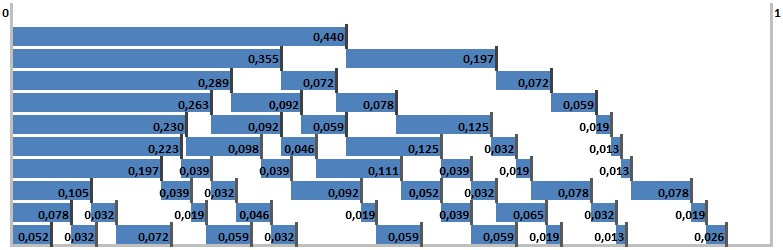
\includegraphics[scale=.7]{sections/images/consciousness_logical_moments.jpg}
\floatfoot{Exemplo de um intervalo lógico com dez momentos lógicos.}%\footnotemark}
\end{figure}
%\footnotetext{Fonte: note}

A consciência são os momentos lógicos de uma expansão representados em suas unidades.
\begin{figure}[H]
\caption{Intervalo lógico consciente}
\label{fig:consciousness}
\centering
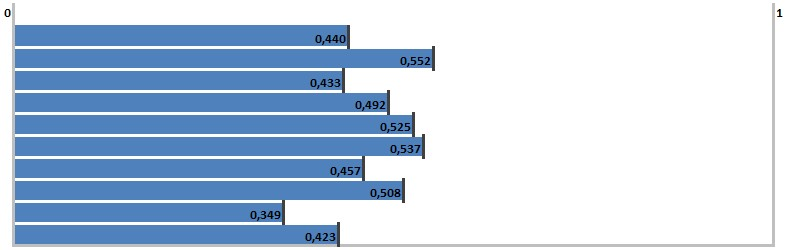
\includegraphics[scale=.7]{sections/images/consciousness.jpg}
\floatfoot{Exemplo de um intervalo lógico consciente com dez unidades de momentos lógicos.}%\footnotemark}
\end{figure}
%\footnotetext{Fonte: note}

Pode ser observado na Tabela \ref{tab:10000_all} que a probabilidade de 99,99\% das amostras, que aumentam em quantidade a medida que crescem os momentos lógicos, tendem a estar cada vez mais ao centro do intervalo lógico, sendo que essa centralização tende ao infinito.
\begin{figure}[H]
\caption{Centralização de 99,99\% das amostras}
\label{fig:centering_of_99_range}
\centering
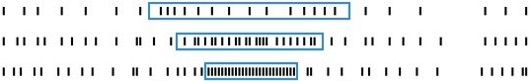
\includegraphics[scale=1]{sections/images/centering_of_99_range.jpg}
\floatfoot{Tendência de centralização do range de 99,99\% das amostras.}%\footnotemark}
\end{figure}
%\footnotetext{Fonte: note}

A consciência é o conjunto dos momentos lógicos unificados de uma expansão. É o aspecto da lógica que unifica as amostras desses momentos, ou seja, é a lógica que abstrai muitos em um, muitas subunidades em uma unidade por momento lógico. Todos os aspectos listados abaixo são inerentes a abstração da lógica chamada consciência.

\subsubsection{Infinito}
Um dos aspectos mais importantes que a negação do nada traz (negação de si), é o infinito, ou seja, em qualquer intervalo lógico cabe o infinito novamente. A lógica primordial que iniciou todo o intervalo lógico é a mesma encontrada em seus intervalos subsequentes. Isso fundamenta como uma lógica de alto nível como a subconsciência humana explica a lógica primordial, uma vez que não é preciso voltar ao primeiro momento lógico do intervalo para deduzi-lo, pois esse fenômeno é onipresente em todo o intervalo.

\subsubsection{Ondas}
Probabilisticamente a distribuição de novas amostras de uma população tendem a concentrar mais amostras sentido a mediana da população com frequências de amostras cada vez maiores neste sentido. Porém, a distribuição dessas amostras com frequências de crescimento uniformes é infinitesimal se comparado às possibilidades randômicas desse crescimento. Assim, a tendência de crescimento dessas frequências sentido a mediana somadas a baixíssima probabilidade (infinitesimal) desse crescimento ser uniforme, conduz a frequências no padrão de ondas.
\begin{figure}[H]
\caption{Padrão de onda}
\label{fig:consciousness_waves}
\centering
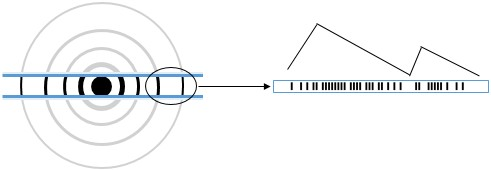
\includegraphics[scale=1]{sections/images/consciousness_waves.jpg}
\floatfoot{Padrão de onda inferido pela tendência dessa distribuição com frequências maiores sentido a mediana da população e a baixíssima probabilidade de crescimento uniforme dessas frequências.}%\footnotemark}
\end{figure}
%\footnotetext{Fonte: note}

Grandes intervalos com baixas frequências de amostras ou grandes intervalos com frequências uniformes de amostras são mais difíceis de observar devido à ausência de grandes discrepâncias. A junção de duas ondas além de eliminar suas discrepâncias, faz com que a primeira onda da união fique maior e a segunda onda acabe por deixar de existir a se tornar parte da primeira, que tem seu pico mais próximo da mediana. Probabilisticamente uma onda não morre, apenas une-se com outras ondas mais internas a ela.
\begin{figure}[H]
\caption{Unificação de ondas}
\label{fig:consciousness_uniform_wave}
\centering
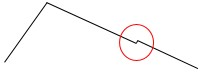
\includegraphics[scale=1]{sections/images/consciousness_uniform_wave.jpg}
\floatfoot{Ondas sendo unificadas para exemplificar o crescimento amostral uniforme.}%\footnotemark}
\end{figure}
%\footnotetext{Fonte: note}

\subsubsubsection{Entrelaçamento e subconsciente}
As amostras que mais se parecem em termos de frequências e distribuição são as amostras que fazem parte da mesma onda. Elas são frequências opostas não sobrepostas que se completam.

Probabilisticamente as duas partes complementares de uma onda estarão a uma distância aproximadamente iguais, equidistante da mediana, porém essa não é uma regra e as partes complementares de uma onda podem estar em distâncias diferentes da mediana. O fenômeno da paridade das partes de uma onda tem o nome de entrelaçamento quântico.

Essas ondas formas subconsciência de uma consciência maior. A consciência é única para todo o intervalo, é a lógica do intervalo, enquanto forma subconsciências, como pequenas ondas de uma onda maior. Assim, uma mudança na onda maior (consciência) também é uma mudança na onda menor (subconsciência), mudança essa que é induzida pela subconsciência indiretamente, análogo ao comprimir gás em um cilindro, que ao adicionar uma nova molécula de gás no cilindro parcialmente cheio, mais próximas ou apertas as moléculas dentro dele estarão. O contrário também é verdadeiro, uma nova amostra em uma subconsciência, que por esta é observada diretamente é também uma mudança da consciência e vai ser induzida por outras subconsciências indiretamente.
\begin{figure}[H]
\caption{Subconsciência}
\label{fig:consciousness_subconscious}
\centering
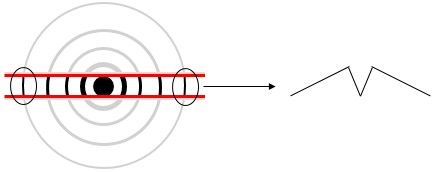
\includegraphics[scale=1]{sections/images/consciousness_subconscious.jpg}
\floatfoot{O padrão de ondas forma subconsciências semelhantes ao padrão criado pela consciência como visto na Figura \ref{fig:statisticsbyjim_central_limit_theorem} ou na Figura \ref{fig:trend_chart_of_normal_distribution}.}%\footnotemark}
\end{figure}
%\footnotetext{Fonte: note}

\subsubsubsection{Salto}
O salto quântico é uma reordenação feita pelo entrelaçamento quântico a medida que as amostras dos agrupamentos mudam com a adição de novas amostras.

Um agrupamento é o range de ondas que uma subconsciência é capaz de observar. E esse range de ondas depende do range de ondas que a própria subconsciência é constituída. Por exemplo, ao observar um grande agrupamento, como o planeta terra, não é possível observar seus detalhes.
\begin{figure}[H]
\caption{Agrupamento subconsciente}
\label{fig:consciousness_space_subconscious_grouping}
\centering
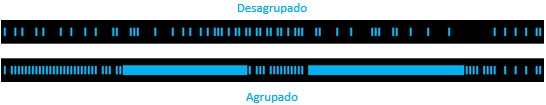
\includegraphics[scale=.8]{sections/images/consciousness_space_subconscious_grouping.jpg}
\floatfoot{Agrupamento de ondas dependente do range de ondas que a própria subconsciência é constituída.}%\footnotemark}
\end{figure}
%\footnotetext{Fonte: note}

Na Figura \ref{fig:consciousness_space_subconscious_observation_jump} ser observado os agrupamentos (colunas do histograma, que nada mais são que subintervalos de uma população na vertical) e reordenação feita pelo entrelaçamento quântico que provoca um salto nas coordenadas (X, Y e Z) conforme subseção do Espaço.
\begin{figure}[H]
\caption{Reordenação subconsciente - Salto}
\label{fig:consciousness_space_subconscious_observation_jump}
\centering
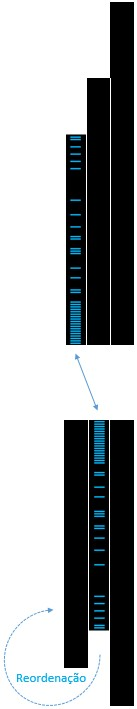
\includegraphics[scale=.6]{sections/images/consciousness_space_subconscious_observation_jump.jpg}
\floatfoot{Salto provocado pelo entrelaçamento.}%\footnotemark}
\end{figure}
%\footnotetext{Fonte: note}

Talvez em experimentos esse salto dure pouco tempo devido a carga de partículas, como o fóton, ser exagerada. Assim o entrelaçamento ocorre e em seguida mais amostras são adicionadas no agrupamento desfazendo a reordenação. 

\subsubsection{Tempo}
O tempo é a adição de novos momento lógicos entre momentos existentes à medida que prossegue a negação de si da lógica. Essas mudanças são acumulativas e a medida que aumentam o número desses momentos lógicos, menos relevante cada novo momento será dentro do intervalo consciente. Um em cem é mais relevante do que um em mil. 
\begin{figure}[H]
\caption{Tempo}
\label{fig:consciousness_time}
\centering
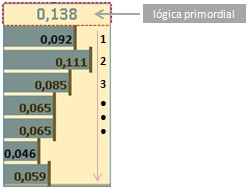
\includegraphics[scale=.8]{sections/images/consciousness_time.jpg}
\floatfoot{Progressão do tempo conforme os momentos lógicos avançam.}%\footnotemark}
\end{figure}
%\footnotetext{Fonte: note}

Outro fator importante a observar do tempo é que, probabilisticamente, subconsciências mais próximas da mediana da população terão uma adição maior de novas amostras em seus intervalos, o que são observados diretamente por essas subconsciências. Por outro lado, subconsciências distantes da mediana da população terão uma adição menor de amostras em seus intervalos e sujeitam-se a um número maior de mudança induzidas indiretamente. Esse fenômeno de observação temporal proporcionado pela consciência e subconsciências evita o paradoxo dos gêmeos \cite{brasilescola_paradoxo_gemeos}.

Na seção Expansão binomial foi apresentado que a lógica é uma sequência de negações de si no tempo zero, ou seja, em nenhum momento entre suas negações a lógica passa a SER, garantindo a premissa primordial da constante lógica, NÃO SER. Assim, a lógica é uma sequência infinita e simultânea, uma constante.
Logo, o tempo é apenas uma grandeza da consciência oriunda da ordenação dessa sequência lógica, não da sequência propriamente. A simultaneidade dessa sequência torna a lógica uma constante com todas as suas infinitas possibilidades, sendo esse universo uma delas. Cada universo tem sua sequência de mudanças, que é estática, em uma ordem diferente e é essa ordem que dá origem à grandeza que chamamos de tempo. É essa ordem do universo ou consciência que vai dar a noção do que acontece antes ou depois, ou seja, o passado, o presente e o futuro.
Na experiência do tempo conduzida pela consciência a ordenação da sequência é a essência dessa grandeza e, portanto, mais relevante do que sua origem que é de natureza simultânea.

\subsubsection{Espaço}
As ondas da consciência exibidas em forma de histograma, onde as partes das ondas que se completam são colocados lado a lodo é exibida na Figura \ref{fig:consciousness_space_waves}. A formação desse histograma é proveniente do entrelaçamento quântico.
\begin{figure}[H]
\caption{Histograma proveniente do entrelaçamento quântico}
\label{fig:consciousness_space_waves}
\centering
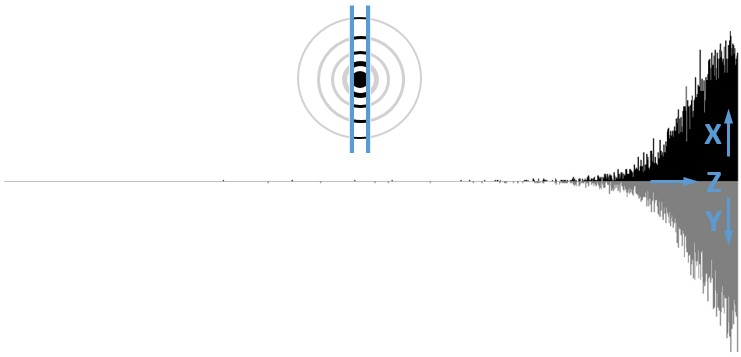
\includegraphics[scale=.7]{sections/images/consciousness_space_waves.jpg}
\floatfoot{Exemplo de padrão de ondas obtido pelo algoritmo Logic\_WavePattern \footnotemark.}
\end{figure}
\footnotetext{O algoritmo Logic\_WavePattern pode ser visto no Apêndice \ref{app:algoritmos}.}

Ao representar as grandezas espaciais conforme o gráfico da Figura \ref{fig:consciousness_space_waves} e distribuir seus pontos de extremidade (desprezando seus volumes e possíveis pontos internos) em um gráfico de distribuição 3D, obtém-se algo parecido com uma espiral (como redemoinhos no ar ou na água) mesmo em volumes muito pequenos de dados (momentos lógicos), conforme Figuras \ref{fig:consciousness_space_3DScatter15000-10} e \ref{fig:consciousness_space_3DScatter_200000-2}. Esses redemoinhos se movem lateralmente, uma vez que as coordenadas X e Y aumentam à medida que novas amostras são adicionadas na população. 
\begin{figure}[H]
\centering
	\begin{subfigure}[H]{0.47\linewidth}
	\centering
	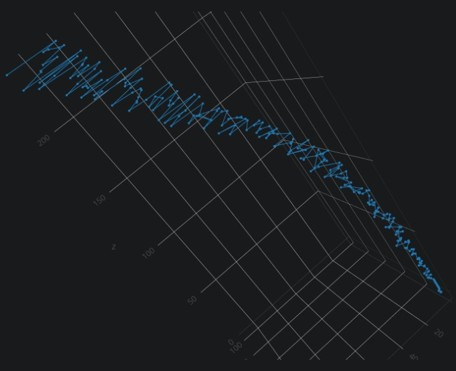
\includegraphics[width=.96\linewidth]{sections/images/consciousness_space_3DScatter15000-10.jpg}
	\caption{15.000 Amostras}
	\label{fig:consciousness_space_3DScatter15000-10}
	\end{subfigure}
\hfill
	\begin{subfigure}[H]{0.47\linewidth}
	\centering
	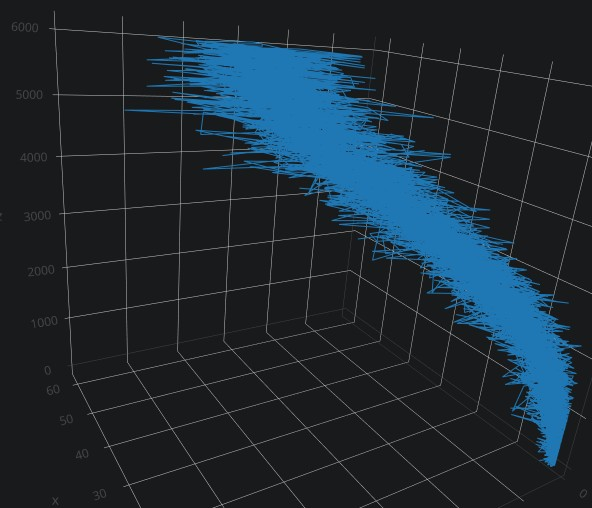
\includegraphics[width=.9\linewidth]{sections/images/consciousness_space_3DScatter_200000-2.jpg}
	\caption{200.000 Amostras}
	\label{fig:consciousness_space_3DScatter_200000-2}
	\end{subfigure}%
\caption{Gráfico de dispersão 3D gerado com os pontos da Figura \ref{fig:consciousness_space_waves}}
\floatfoot{O histograma no padrão de ondas e os dados para gerar o gráfico de dispersão 3D podem ser obtidos com a execução do algoritimo Logic\_WavePattern \protect\footnotemark.}
\end{figure}
\footnotetext{O algoritmo Logic\_WavePattern pode ser visto no Apêndice \ref{app:algoritmos} e os gráficos de dispersão 3D podem ser acessados em: \url{https://chart-studio.plot.ly/create/?fid=ren.stuchi:5&fid=ren.stuchi:4} e \url{https://chart-studio.plot.ly/create/?fid=ren.stuchi:7&fid=ren.stuchi:6}}

A observação de outras subconsciências depende do range de ondas que uma subconsciência é capaz de observar e esse range, por sua vez depende do range de ondas que a própria subconsciência é constituída.

Em agrupamentos de muitos momentos lógicos pode-se ver o agrupamento de grandes objetos (subconsciências), sendo o maior deles representado pela cor azul claro e os menores e mais distantes pela cor azul escuro ou roxo, conforme Figura \ref{fig:consciousness_space_subconsciousness}. Esse agrupamento pode representar, por exemplo, o centro do universo, então o centro de uma galáxia, estrelas, planetas e objetos menores e mais distantes.
\begin{figure}[H]
\caption{Abstração espacial das subconsciências - grandes agrupamentos}
\label{fig:consciousness_space_subconsciousness}
\centering
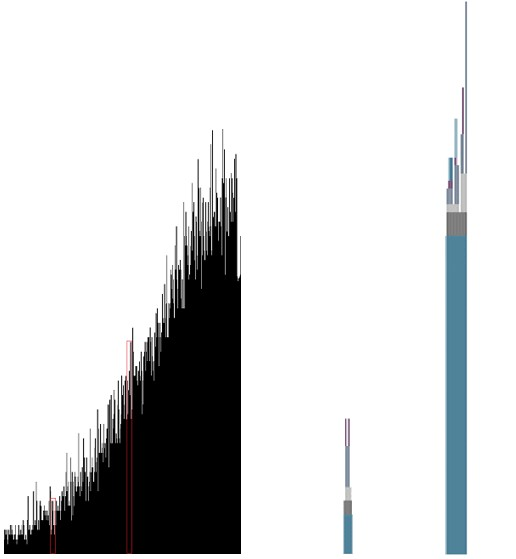
\includegraphics[scale=.5]{sections/images/consciousness_space_subconsciousness.jpg}
\floatfoot{Caracteristicas da ondas formadoras da subconsciência de grandes objetos.}%\footnotemark}
\end{figure}
%\footnotetext{Fonte: note}

Em agrupamentos com uma quantidade menor de momentos lógicos pode-se ver o agrupamento de pequenos objetos (subconsciências). Quanto menores os agrupamentos menos divisões esses agrupamentos têm (cores) e mais estreitos e compridos eles são, conforme Figura \ref{fig:consciousness_space_subconsciousness_min}. Esse agrupamento pode representar, por exemplo, o átomo que são muito pequenos, se apresentam em enormes quantidades e as partículas que orbitam seu núcleo (elétrons) ficam bem mais distantes dele.
\begin{figure}[H]
\caption{Abstração espacial das subconsciências - pequenos agrupamentos}
\label{fig:consciousness_space_subconsciousness_min}
\centering

\includegraphics[scale=.9]{sections/images/consciousness_space_subconsciousness_min.jpg}
\floatfoot{Caracteristicas da ondas formadoras da subconsciência de pequenas partículas.}%\footnotemark}
\end{figure}
%\footnotetext{Fonte: note}}

\begin{description}
   \item[Espiral] Provavelmente, o padrão aproximado de espiral, visto nas Figuras \ref{fig:consciousness_space_3DScatter15000-10} e \ref{fig:consciousness_space_3DScatter_200000-2}, refletirão das primeiras consciências (azul claro) para as demais, pois estas são partes das primeiras e assim por diante;
   \item[Eixos X e Y] A consciência e suas subconsciências são uma mixagem dois eixos X e Y;
   \item[Volume] O volume dobra a cada um terço de crescimento das colunas do histograma, aproximadamente. Como exibido na Figura \ref{fig:consciousness_dark_matter_dark_energy_wave}, os momentos lógicos ficam mais concentrados no começo das ondas entrelaçadas, o que pode gerar algo de facíl observação nessa região, como estrelas, planetas etc. 
\end{description}

\subsubsection{Forças fundamentais}
A força gravitacional, a força eletromagnética e a força nuclear correspondem às forças fundamentais da natureza e essas forças também são provenientes do entrelaçamento quântico, como o espaço. As forças fundamentais não são forças propriamente, mas sim aspectos probabilísticos (distribuição normal) e do entrelaçamento de ondas principalmente.

\subsubsubsection{Força gravitacional}
O entrelaçamento quântico, que define os pares de ondas opostas não sobrepostas que se completam e que mais se assemelham em termos de frequência e distribuição das amostras, é o aspecto que coordena as mudanças nas coordenadas espaciais. As mudanças dessas coordenadas provocam iterações que podem ser vistas nas Figuras \ref{fig:consciousness_space_3DScatter15000-10} e \ref{fig:consciousness_space_3DScatter_200000-2} da subseção de Espaço. Essas iterações são chamadas de gravidade.

\subsubsubsection{Força eletromagnética}
A força eletromagnética é uma especificação do aspecto gravitacional que depende da aproximação espacial (redução de diferenças nos eixos X, Y e Z) e do entrelaçamento quântico.

Quando um objeto se aproxima de outro, seus pares de ondas provenientes do entrelaçamento quântico ficam cada vez mais parecidos, eixos X e Y. Essa proximidade faz com que as partes das ondas de um objeto se pareça muito com as partes das ondas do outro objeto, o que pode fazer com que o entrelaçamento quântico encontre pares mais ideais nesse outro objeto e vice-versa.  

As linhas azuis da Figura \ref{fig:consciousness_electromaagnetic_force} mostra onde é mais frequente a troca dos pares de ondas pelo entrelaçamento quântico, ou seja, onde se tem a maior probabilidade das ondas serem parecidas. Por isso os imãs tentam se virar para se conectar quando estão face a face com o mesmo polo. As linhas cinza mostram as conexões que ocorrem em número bem menor. 
\begin{figure}[H]
\caption{Força eletromagnética}
\label{fig:consciousness_electromaagnetic_force}
\centering
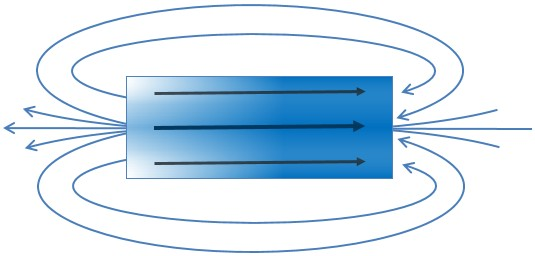
\includegraphics[scale=.6]{sections/images/consciousness_electromaagnetic_force.jpg}
\floatfoot{Aumento das possibilidades de entrelaçamento quântico devida a aproximação e menor número de momentos lógicos das menores partículas. }%\footnotemark}
\end{figure}
%\footnotetext{Fonte: note}

Com a troca de significativos pares de ondas entre os objetos faz-se a mixagem do posicionamento dos eixos X, Y e Z entre esses objetos ocorrendo a aproximação deles no espaço. 

Quanto menor a partícula (elétron ou partículas menores), conforme Figura \ref{fig:consciousness_space_subconsciousness_min}, mais fácil o entrelaçamento ocorre. Provavelmente muitos objetos não tenham alta capacidade de entrelaçamento devido aos seus elétrons ou partículas menores serem formadas por muitos momentos lógicos (barras do histograma mais largas ou mais compridas), ou seja, quanto maior a quantidade de momentos dessas partículas menores as chances de entrelaçamento.

Probabilisticamente as partículas mais parecidas estão nas regiões mais próximas (linhas azuis do Figura \ref{fig:consciousness_electromaagnetic_force}), porém isso não é uma regra e os polos podem se inverter, ou seja, ter mais ligações com a região de menor probabilidade (isso não quer dizer que houve formação de antimatéria nessa região, as particulas tendem a concetrar mais momentos lógicos sentido à mediana da população). No entanto, a probabilidade tende a corrigir esses polos conforme novos momentos vão sendo adicionadas nesse intervalo. 

\subsubsubsection{força nuclear}
As forças nucleares forte e fraca representam as maiores concentrações de momentos lógicos por intervalo populacional. Esses picos podem ser vistos na Figura \ref{fig:consciousness_space_subconsciousness_min} e eles não param de crescer à medida que novos momentos lógicos são adicionados nestes intervalos. Estes momentos tendem a estarem cada vez mais juntos dentro do intervalo formando picos cada vez mais altos, ou seja, há uma crescente frequência de ondas nesses pequenos intervalos.

\subsubsection{Matéria escura e energia escura}
Quanto maior o número de amostras e mais próximas elas estão da mediana, mais elas farão parte dos 99,99\% e ainda mais amostras também estarão nos 0,01\%, conforme a Tabela \ref{tab:10000_all}.
\begin{figure}[H]
\centering
	\begin{subfigure}[H]{1\linewidth}
	\centering
	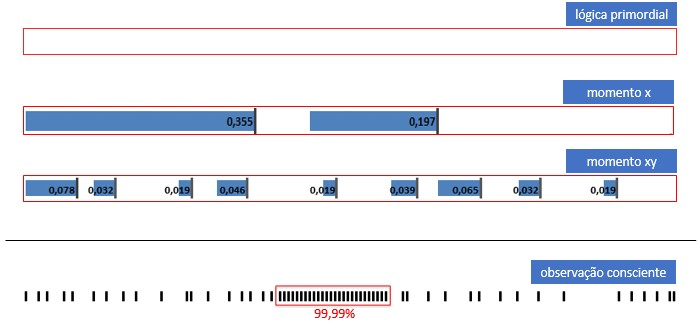
\includegraphics[width=.76\linewidth]{sections/images/consciousness_dark_matter_dark_energy.jpg}
	\caption{}
	\label{fig:consciousness_dark_matter_dark_energy}
	\end{subfigure}
\hfill
	\begin{subfigure}[H]{0.7\linewidth}
	\centering
	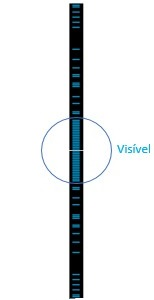
\includegraphics[width=.3\linewidth]{sections/images/consciousness_dark_matter_dark_energy_wave.jpg}
	\caption{}
	\label{fig:consciousness_dark_matter_dark_energy_wave}
	\end{subfigure}%
\caption{Analogia da matéria escura}
\floatfoot{Volume facilmente observado por outras subconsciências.} %\protect\footnotemark.}
\end{figure}
%\footnotetext{}

A Figura \ref{fig:consciousness_dark_matter_dark_energy_wave} mostra probabilisticamente onde está a maior concentração das amostras de um intervalo, tornando mais fácil a visualização por outras subconsciências, uma vez que o volume dobra a cada um terço do crescimento das colunas do histograma, aproximadamente.

A energia escura não é uma energia propriamente, mas sim aspectos do entrelaçamento de ondas, como as forças fundamentais da natureza e o espaço, conforme Figuras \ref{fig:consciousness_space_waves} e \ref{fig:consciousness_space_3DScatter_200000-2}

\subsubsection{Antimatéria}
Independente do intervalo observado, sua maior concentração de amostras tende a estar sentido da mediana, o que é o sentido provável conforme teorema central do limite. Essas amostras também podem estar com sua concentração no sentido oposto à mediana, porém com uma ocorrência probabilística cada vez menos conforme as amostras aumentam. Na Figura \ref{fig:consciousness_concentration_of_opposite_samples} é exibido dois intervalos idênticos com suas amostras com concentrações opostas.
\begin{figure}[H]
\caption{Parte de um intervalo idêntico com suas concentrações de amostras opostas}
\label{fig:consciousness_concentration_of_opposite_samples}
\centering
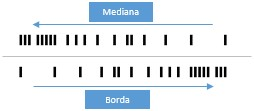
\includegraphics[scale=1]{sections/images/consciousness_concentration_of_opposite_samples.jpg}
\floatfoot{Parte de um intervalo idêntico distribuídos de formas opostas.}%\footnotemark}
\end{figure}
%\footnotetext{Fonte: note}

O merge ou soma dos intervalos opostos da Figura \ref{fig:consciousness_concentration_of_opposite_samples} os tornaria um intervalo simétrico, ou seja, não estaria em nenhum dos sentidos.
Na Figura \ref{fig:consciousness_concentration_of_opposite_samples_within_range} é exibido um intervalo consciente completo com suas concentrações de amostras sentido à mediana e outro idêntico, mas com suas concentrações sentido às bordas do intervalo.
\begin{figure}[H]
\caption{Intervalos conscientes com suas concentrações de amostras opostas}
\label{fig:consciousness_concentration_of_opposite_samples_within_range}
\centering
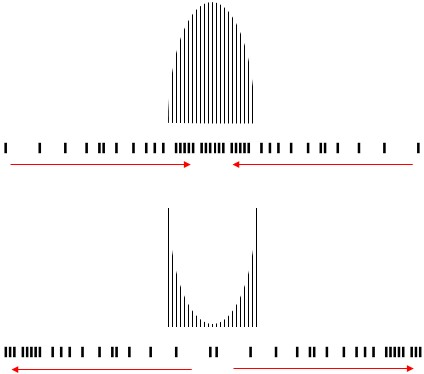
\includegraphics[scale=.8]{sections/images/consciousness_concentration_of_opposite_samples_within_range.jpg}
\floatfoot{Intervalos conscientes completos e idênticos distribuídos de formas opostas.}%\footnotemark}
\end{figure}
%\footnotetext{Fonte: note}


\subsubsection{Buraco negro}
O buraco negro é uma concentração muito alta de amostras, formada por grandes agrupamentos subconscientes, Figura \ref{fig:consciousness_space_subconsciousness}.
Esses grandes agrupamentos ocupam grandes volumes de espaço devido a quantidade de amostras. 

Os grandes volumes são encontrados na base dos grandes agrupamentos, conforme as cores azul claro e cinza da Figura \ref{fig:consciousness_black_hole}.
\begin{figure}[H]
\caption{Buracos negros}
\label{fig:consciousness_black_hole}
\centering
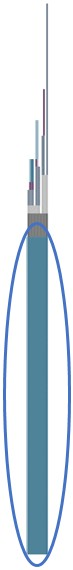
\includegraphics[scale=.6]{sections/images/consciousness_black_hole.jpg}
\floatfoot{Grandes volumes são encontrados na base dos grandes agrupamentos.}%\footnotemark}
\end{figure}
%\footnotetext{Fonte: note}